\documentclass{beamer}
\setbeamertemplate{navigation symbols}{}
\setbeamertemplate{footline}{}
\usepackage[utf8]{inputenc}
\usepackage{utopia} %font utopia imported
\usetheme{Berlin}
\definecolor{UBCblue}{rgb}{0.04706, 0.13725, 0.26667} % UBC Blue (primary)

\usecolortheme[named=UBCblue]{structure}%------------------------------------------------------------
\title[MAP 3305] %optional
{How Tesla's AI utilizes differential equations}



\author[Cattan, Dov] % (optional)
{Dov Cattan}

\institute[FAU] % (optional)
{
  
  Student, Computer Engineering\\
  Florida Atlantic University
  
}

\date[ 2022] 
{
 Engineering Math, Spring 2022
\newline \newline  TWO MINUTE VIDEO REFERENCE: https://www.youtube.com/watch?v=6hkiTejoyms
}




\begin{document}
\frame{\titlepage}

\section{}


\begin{frame}
\frametitle{How does Tesla's AI figure out how to self drive}
In order to have the car to navigate properly on it's own, the car is given the correct speed and acceleration to the correct position. \newline


   
    Speed: $\frac{dx}{dt}$,$\frac{dy}{dt}$, $\frac{dz}{dt} = x, y, z$.         
    Acceleration: $\frac{d^2x}{dt^2}$,$\frac{d^2y}{dt^2}$,$\frac{d^2z}{dt^2} = x, y, z$.
   \newline
   


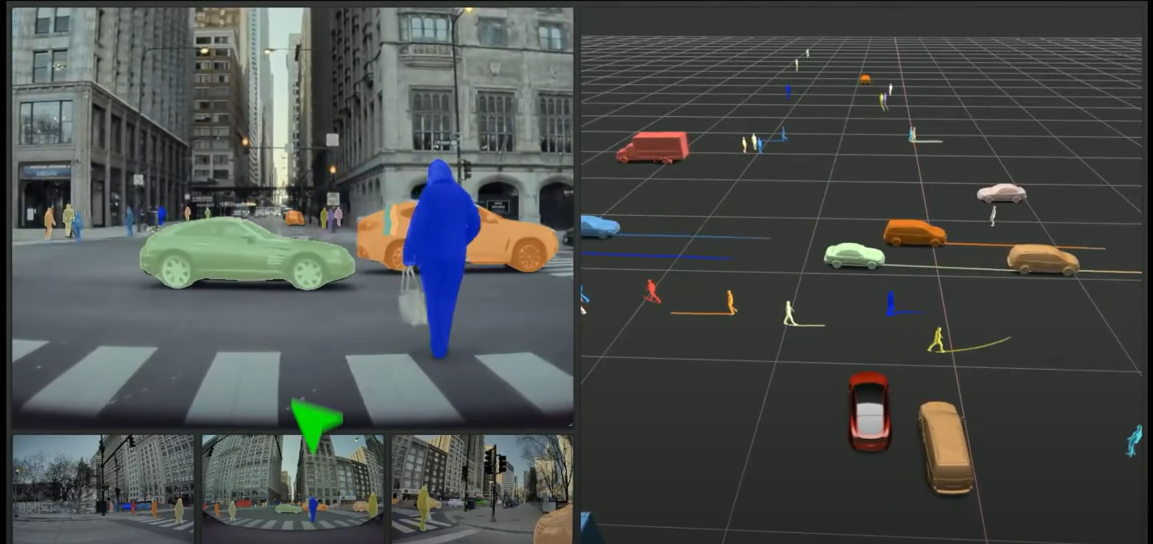
\includegraphics[height = 4.35cm, width= \textwidth]{tesla 1.PNG}

\end{frame}



\section{}
%---------------------------------------------------------
%Highlighting text
\begin{frame}
\frametitle{How to find the rate of change with the depth and velocity of Tesla's AI}

The data below is the rate of change of the velocity and depth that was needed to navigate the area the car was driving in using cameras.
\newline

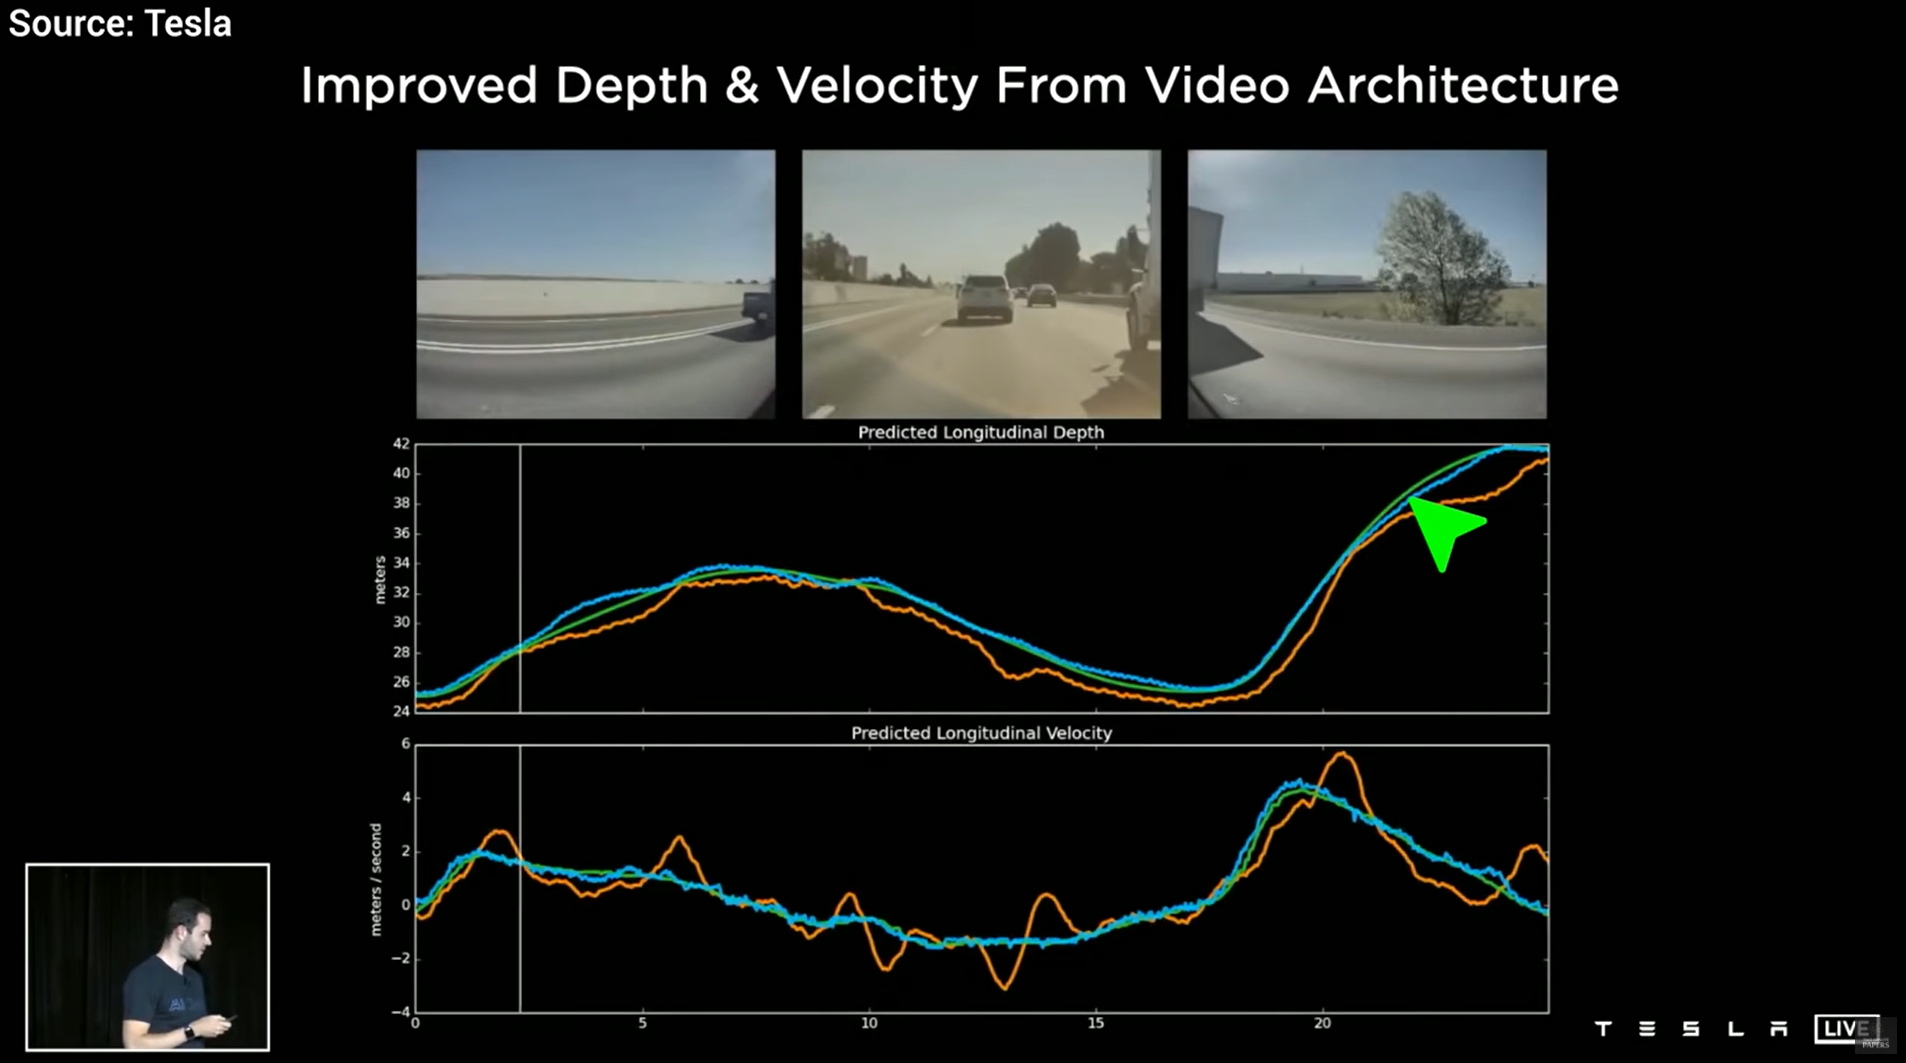
\includegraphics[height=4.32cm,width = 9cm]{tesla 2.PNG}\centering




\end{frame}
%---------------------------------------------------------


%---------------------------------------------------------
%Two columns
\begin{frame}
\frametitle{Obstacle detection}




When the cameras detect and avoid other cars, building, people, or other obstacles, speed and acceleration must increase or decrease at very high rates during minuscule changes of time.
\newline



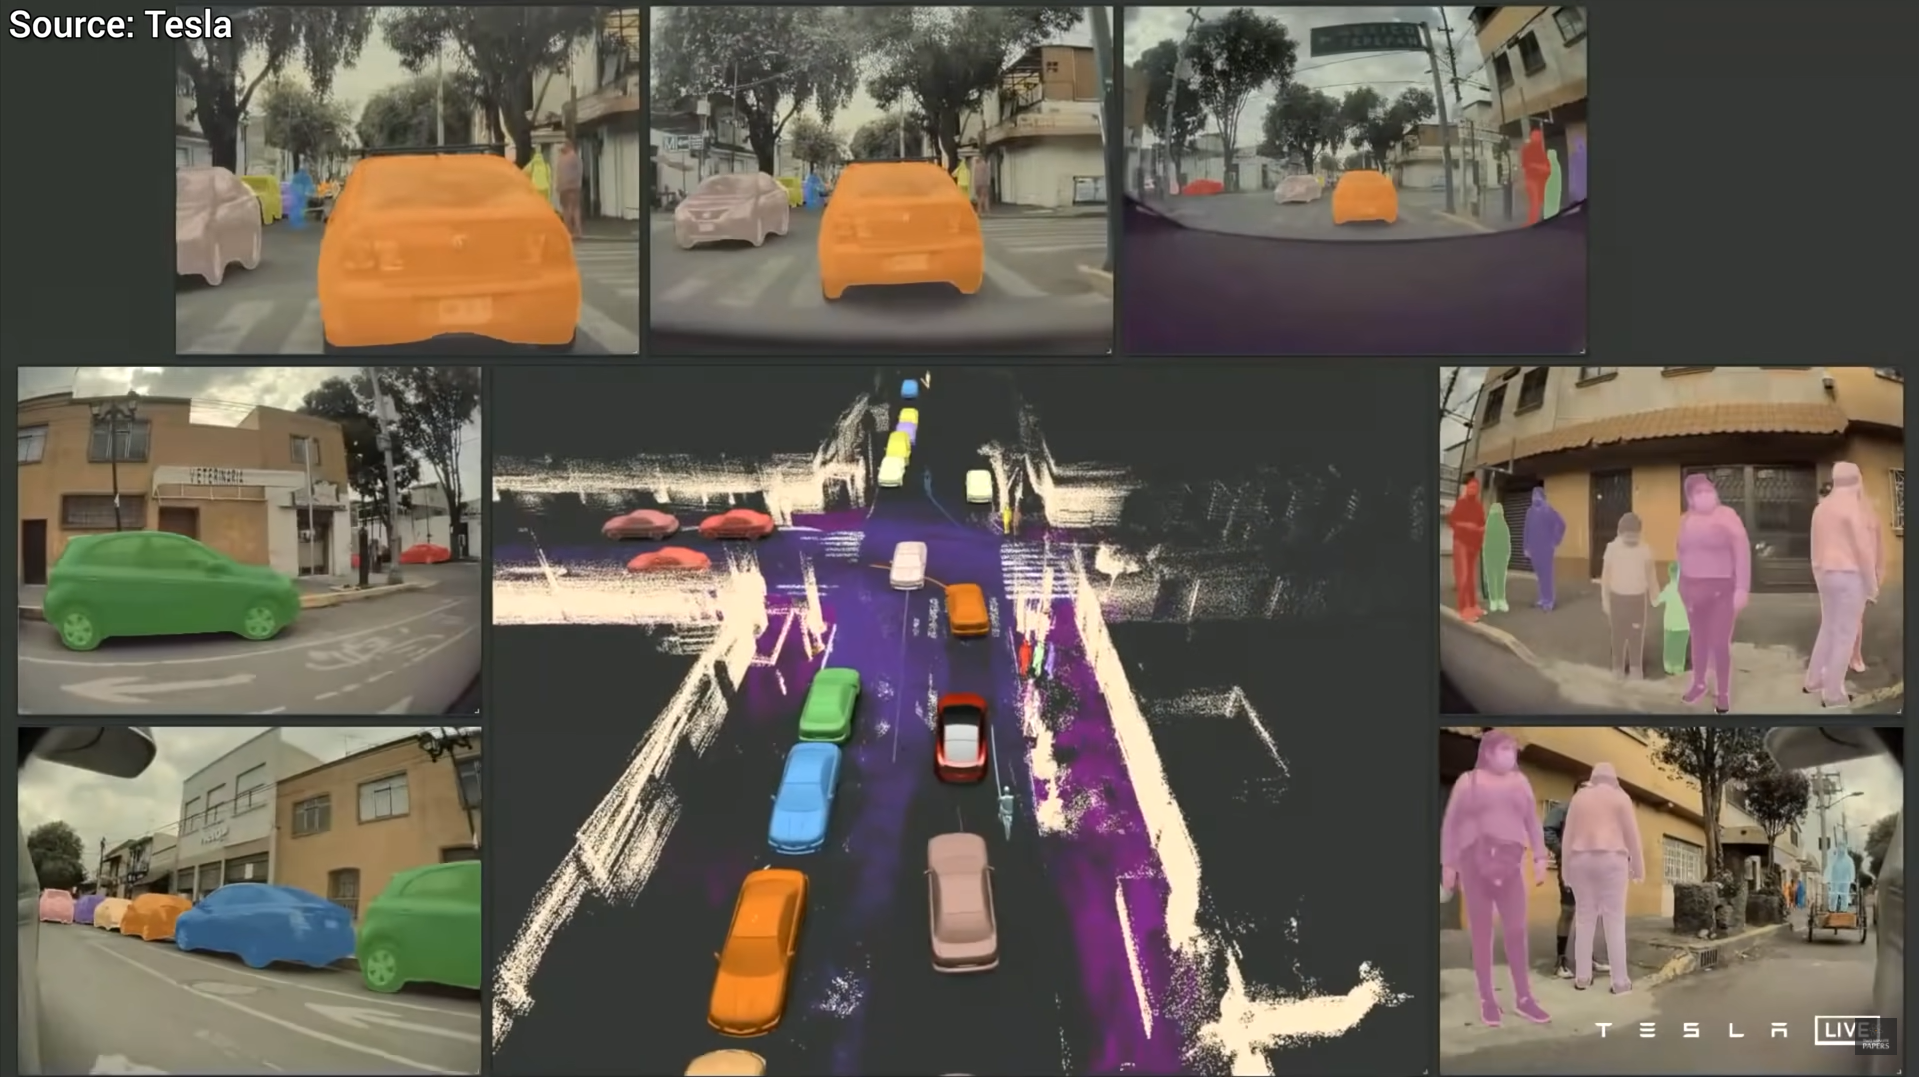
\includegraphics[height=4.9cm,width = \textwidth]{tesla 3.PNG}

\end{frame}
%---------------------------------------------------------


\end{document}
